\documentclass[11pt]{article}

\usepackage{graphicx}
\usepackage[margin=1in]{geometry}
\usepackage{fancyhdr}
\usepackage[brazilian]{babel}
\usepackage[utf8]{inputenc}
\usepackage[T1]{fontenc}
\usepackage{url}
\usepackage{cite}
\usepackage{indentfirst}
\usepackage{ragged2e}
\usepackage{float}

\setlength\RaggedRightParindent{15pt}

\setlength\parindent{24pt}
\setlength{\parskip}{5pt plus 1pt}
\setlength{\headheight}{13.6pt}

\newcommand\question[2]{\vspace{.25in}\hrule\textbf{#1: #2}\vspace{.5em}\hrule\vspace{.10in}}
\renewcommand\part[1]{\vspace{.10in}\textbf{(#1)}}
\pagestyle{fancyplain}
\lhead{\textbf{\NAME\ }}
\chead{\textbf{Detalhamento da proposta}}
\rhead{\today}


\begin{document}\raggedright
%Section A==============Change the values below to match your information==================
\newcommand\NAME{Marcelo G de Andrade}  % your name
\newcommand\HWNUM{1}              % the homework number
%Section B==============Put your answers to the questions below here=======================

% no need to restate the problem --- the graders know which problem is which,
% but replacing "The First Problem" with a short phrase will help you remember
% which problem this is when you read over your homeworks to study.

\question{1}{Projetos Similares}

\RaggedRight
Há muitos projetos envolvendo eletrônicos movidos por atividades cerebrais, mas a maioria foca na tecnologia de leitura dessas atividades do que o sistema embarcado em si. O primeiro exemplo pode ser visto em \cite{brainwaves_project}. Utilizando um arduino, um simples robô, um dispositivo para leitura de atividade cerebral e um circuito externo, foi feito um projeto muito similar a este.

A parte mais interessante desse projeto foi o sensor utilizado. Ele é originalmente um brinquedo, mas foi desmontado para se tornar um ótimo sensor de atividade cerebral com custo baixo, e esse processo é muito bem detalhado. A explicação da teoria científica por trás das atividades cerebrais também é muito clara e simples. Em termos de computação, o projeto deixa a desejar pois utiliza um arduino e não se preocupa muito com os detalhes do sistema periférico, mas mesmo assim, é uma ótima base para o projeto.

O segundo projeto é mais detalhado que o primeiro, um artigo feito somente para o desenvolvimento de robô movido através de atividade cerebrais, como visto em \cite{make_mind_controlled}. Esse artigo explica muito bem o embarcado por trás do robô, a teoria de leitura de atividade cerebral e mostra uma segunda opção de sensor para essa leitura. Por ser um artigo feito especialmente para isso, seu nível de detalhamento é muito maior que o primeiro projeto apresentado, mas complementando as informações apresentadas nos dois projetos, pode-se adquirir conhecimento essencial para o desenvolvimento do projeto proposto.

\raggedright
\question{2}{Diagrama detalhado}

\begin{figure}[h!]
	\centering
	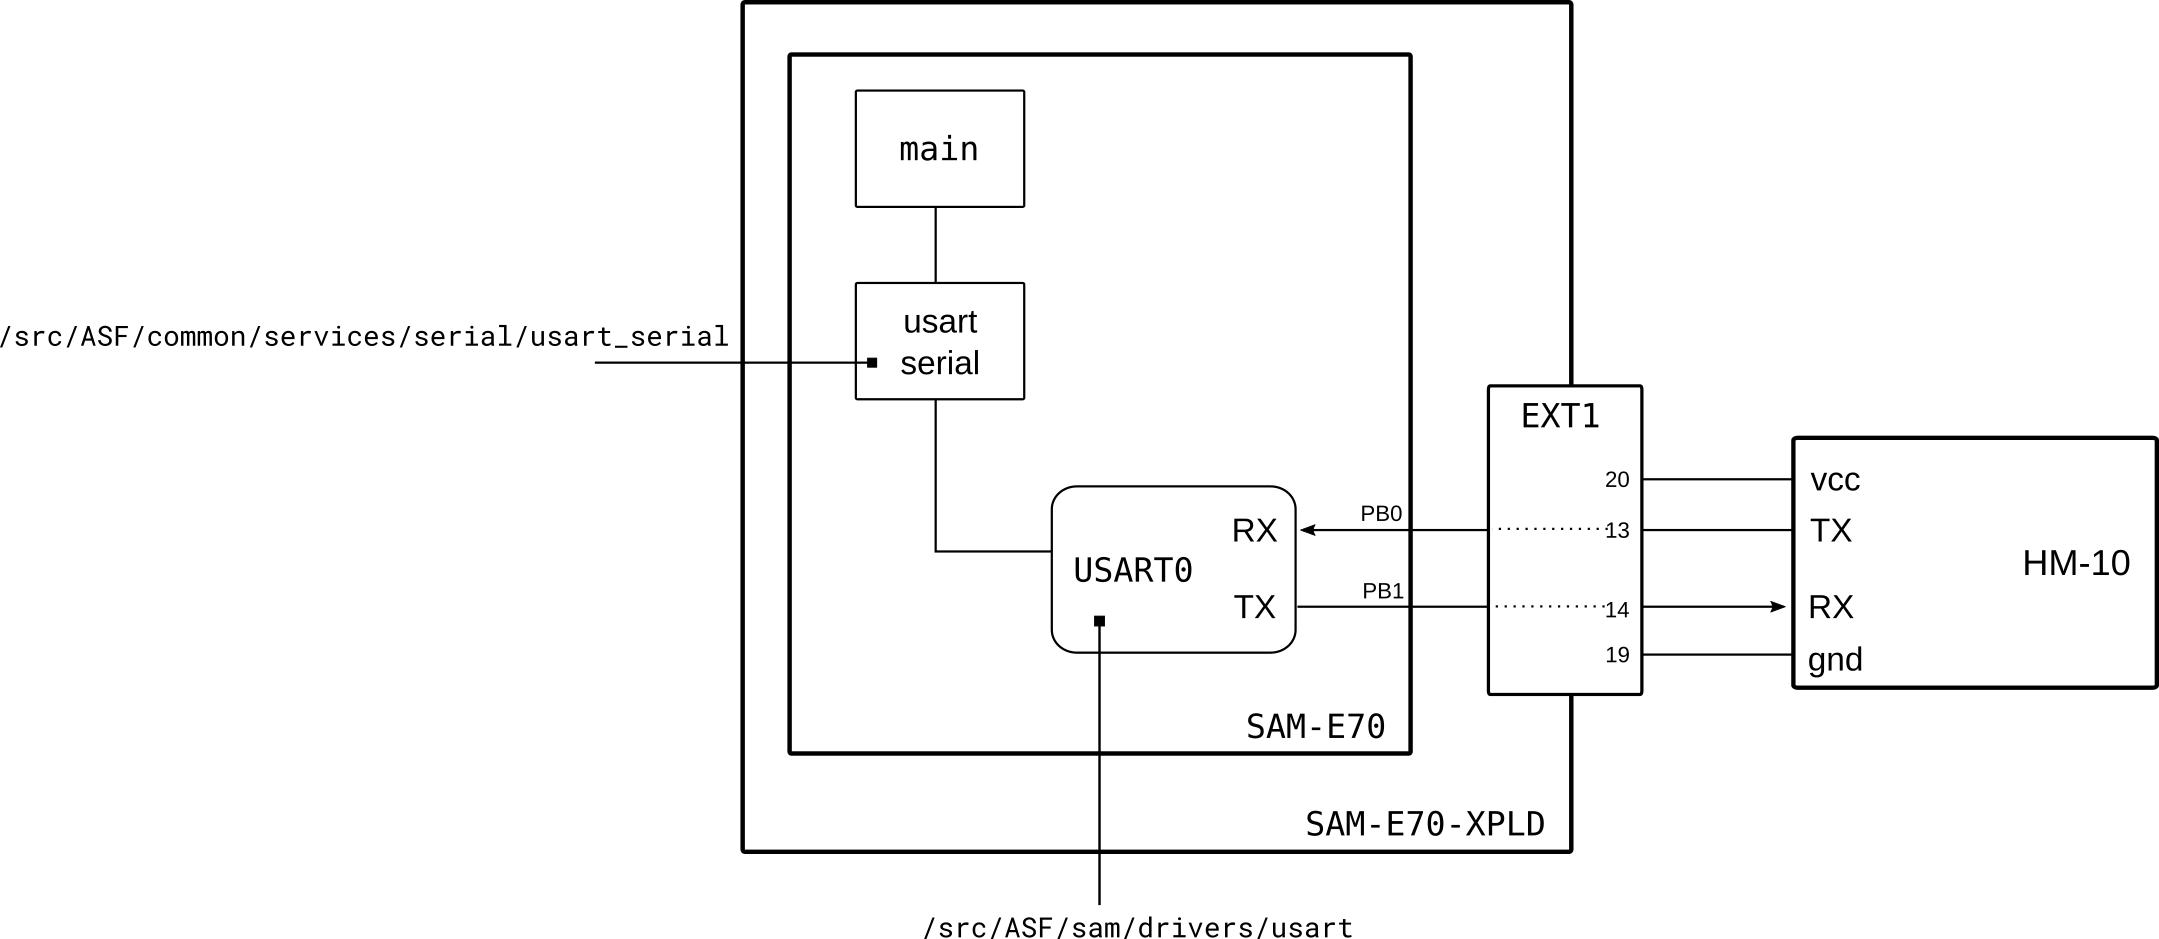
\includegraphics[width=0.7\textwidth]{diagrama.png}
	\caption{Diagrama de blocos.}
\end{figure}


\raggedright
\question{3}{Cronograma de execução simplificado}

O cronograma de execução é o seguinte:

\begin{itemize}
	\item Leitura dos dados pelo sensor de EEG
	\item Filtro dos dados e processamento dentro do processador no sensor
	\item Envio de dados por Bluetooth para o embarcado
	\item Recebimento e tratamento de dados pelo micro processador
	\item Salvar e utilizar dados contidos na memória se necessário
	\item Calculo dos dados e envio de sinal para o motor DC
\end{itemize}

\raggedright
\question{4}{Melhoria no resumo}

\RaggedRight

Esse projeto consiste de um embarcado que se comporta como um pequeno robô/carro e é movido através de atividades cerebrais de um usuário. Um sensor de EEG se comunicará através de uma conexão bluetooth com o embarcado e enviará sinais correspondentes a atividade cerebral de quem utiliza o sensor. Esses sinais serão tratados e analisados pelo microprocessador do embarcado e transformados em sinais para um motor DC que movimentará pequenas rodas, movimentando o embarcado para frente e para trás.

\bibliography{ref}{}
\bibliographystyle{plain}
\end{document}